\documentclass[14pt,compress]{beamer}


% Modified from: generic-ornate-15min-45min.de.tex
\mode<presentation>
{
  \usetheme{Warsaw}
  \useoutertheme{infolines}
  \setbeamercovered{invisible}
}

\usepackage[english]{babel}
\usepackage[latin1]{inputenc}
%\usepackage{times}
\usepackage[T1]{fontenc}

% Taken from Fernando's slides.
\usepackage{ae,aecompl}
\usepackage{mathpazo,courier,euler}
\usepackage[scaled=.95]{helvet}

\definecolor{darkgreen}{rgb}{0,0.5,0}

\usepackage{listings}
\lstset{language=Python,
    basicstyle=\ttfamily\bfseries,
    commentstyle=\color{red}\itshape,
  stringstyle=\color{darkgreen},
  showstringspaces=false,
  keywordstyle=\color{blue}\bfseries}

%%%%%%%%%%%%%%%%%%%%%%%%%%%%%%%%%%%%%%%%%%%%%%%%%%%%%%%%%%%%%%%%%%%%%%
% Macros
\setbeamercolor{emphbar}{bg=blue!20, fg=black}
\newcommand{\emphbar}[1]
{\begin{beamercolorbox}[rounded=true]{emphbar}
      {#1}
 \end{beamercolorbox}
}
\newcounter{time}
\setcounter{time}{0}
\newcommand{\inctime}[1]{\addtocounter{time}{#1}{\tiny \thetime\ m}}

\newcommand{\typ}[1]{\textbf{\texttt{{#1}}}}


\newcommand{\kwrd}[1]{ \texttt{\textbf{\color{blue}{#1}}}  }

%%% This is from Fernando's setup.
% \usepackage{color}
% \definecolor{orange}{cmyk}{0,0.4,0.8,0.2}
% % Use and configure listings package for nicely formatted code
% \usepackage{listings}
% \lstset{
%    language=Python,
%    basicstyle=\small\ttfamily,
%    commentstyle=\ttfamily\color{blue},
%    stringstyle=\ttfamily\color{orange},
%    showstringspaces=false,
%    breaklines=true,
%    postbreak = \space\dots
% }

%\pgfdeclareimage[height=0.75cm]{iitmlogo}{iitmlogo}
%\logo{\pgfuseimage{iitmlogo}}


%% Delete this, if you do not want the table of contents to pop up at
%% the beginning of each subsection:
\AtBeginSubsection[]
{
  \begin{frame}<beamer>
    \frametitle{Outline}
    \tableofcontents[currentsection,currentsubsection]
  \end{frame}
}

\AtBeginSection[]
{
  \begin{frame}<beamer>
    \frametitle{Outline}
    \tableofcontents[currentsection,currentsubsection]
  \end{frame}
}

% If you wish to uncover everything in a step-wise fashion, uncomment
% the following command:
%\beamerdefaultoverlayspecification{<+->}

%\includeonlyframes{current,current1,current2,current3,current4,current5,current6}


\title[Names and Objects]{Advanced Python}
\subtitle{Statements, Expressions, Names, and Objects}

\author[FOSSEE] {The FOSSEE Group}

\institute[IIT Bombay] {Department of Aerospace Engineering\\IIT Bombay}
\date[] {Mumbai, India}

\begin{document}

\begin{frame}
  \titlepage
\end{frame}

\begin{frame}
  \frametitle{Overview}
  \begin{itemize}
  \item Statements
  \item Expressions
  \item Variables
  \item Objects
  \item Names
  \end{itemize}
\end{frame}

\begin{frame}
  \frametitle{Recap of essential concepts}
  \begin{itemize}
  \item Mutable data types
  \item Immutable data types
  \end{itemize}
\end{frame}

\begin{frame}
  \frametitle{Expressions}
  \begin{itemize}
  \item Evaluate to something
  \item Describe some computation
  \item Python evaluates expressions
  \end{itemize}
\end{frame}

\begin{frame}[fragile]
  \frametitle{Examples of Expressions}
  \small
  \begin{lstlisting}
In []: 1
Out[]: 1

In []: (1 + 1.2) * 2.0
Out[]: 4.4

In []: sin(0.1)
Out[]: 0.09983341664682815

In []: (2 > 1) and (3 > 2)
Out[]: True

In []: [1, 2, 3, 4][::2]
Out[]: [1, 3]
# Note that each has an output
  \end{lstlisting}
\end{frame}

\begin{frame}[fragile]
  \frametitle{Statements}
  \begin{itemize}
  \item Instruct Python to perform some action
  \item A program is a series of statements
  \item A statement can have expressions
  \item Assignments are statements
  \end{itemize}
\begin{lstlisting}
In []: a = 1

In []: a += 1
\end{lstlisting}
\end{frame}

\begin{frame}[fragile]
  \frametitle{Assignment statements}
  \begin{lstlisting}
In []: a = 1

In []: a = 'hello'
\end{lstlisting}
\begin{itemize}
\item These are assignment statements
\item Values are \emph{Objects}
\end{itemize}
\end{frame}

\begin{frame}
  \frametitle{Objects}
  \begin{itemize}
  \item Objects: all data in Python
  \item Have an identity, type, and value
  \item Identity is checked using \typ{is}
  \item Identity and type cannot change
  \item Value of mutables change
  \item Immutable object value cannot change
  \end{itemize}
\end{frame}

\begin{frame}[fragile]
  \frametitle{Names and objects}
  \begin{itemize}
  \item Assignment binds a name to an object
  \end{itemize}
  \begin{lstlisting}
In []: a = 1

In []: b = 1
  \end{lstlisting}
  \begin{itemize}
  \item \typ{a} is a name for the object \typ{1}
  \item \typ{b} is also a name for the same object \typ{1}
  \end{itemize}
  \begin{lstlisting}
In []: b = a  # The same as above
\end{lstlisting}
\end{frame}

\begin{frame}[fragile]
  \frametitle{Visualizing this}
  \begin{minipage}{0.4\textwidth}
    \begin{lstlisting}
In []: a = 1
    \end{lstlisting}
  \end{minipage}
  \begin{minipage}{0.4\textwidth}
    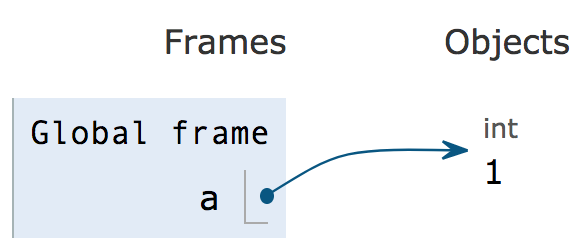
\includegraphics[width=2.5in]{data/a_eq_1.png}
  \end{minipage}
\pause
  \begin{minipage}{0.4\textwidth}
    \begin{lstlisting}
In []: b = a
    \end{lstlisting}
  \end{minipage}
  \begin{minipage}{0.4\textwidth}
    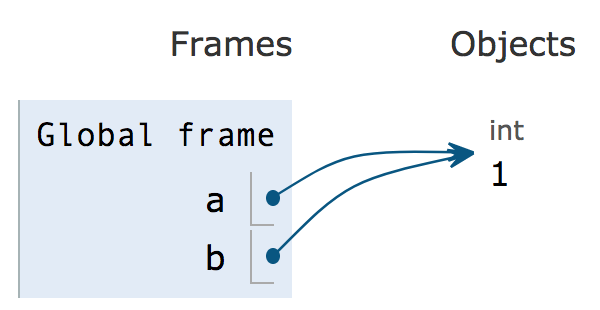
\includegraphics[width=2.5in]{data/a_b_eq_1.png}
  \end{minipage}

  {\small Made with: \url{pythontutor.com}}
\end{frame}

\begin{frame}[fragile]
  \frametitle{Visualizing this ...}
  Set \typ{b} to something else:

  \begin{minipage}{0.4\textwidth}
    \begin{lstlisting}
In []: a = 1

In []: b = 2
    \end{lstlisting}
  \end{minipage}
  \begin{minipage}{0.4\textwidth}
    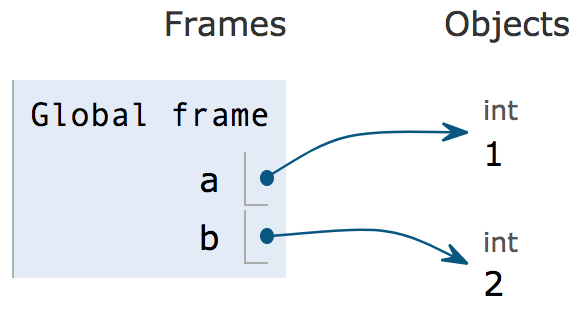
\includegraphics[width=2.5in]{data/a_1_b_2.png}
  \end{minipage}

  \vspace*{1in}
  {\small Made with: \url{pythontutor.com}}
\end{frame}

\begin{frame}[fragile]
  \frametitle{Names and objects ...}
  \begin{itemize}
  \item More interesting when \typ{a} is a list
  \end{itemize}
  \begin{minipage}{0.4\textwidth}
  \begin{lstlisting}
In []: a = [1, 2]
\end{lstlisting}
\end{minipage}
  \begin{minipage}{0.4\textwidth}
    \hspace*{0.2in}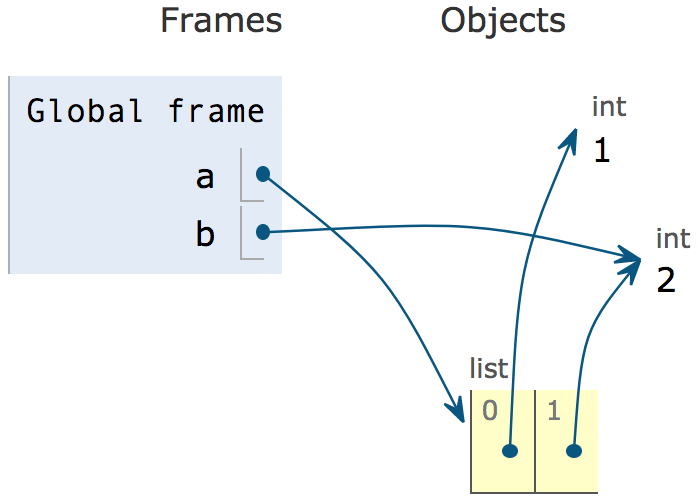
\includegraphics[width=2.25in]{data/a_list_b_2.png}
  \end{minipage}
\end{frame}

\begin{frame}[fragile]
  \frametitle{Names and objects ...}
  \begin{minipage}{0.4\textwidth}
  \begin{lstlisting}
In []: b = a
\end{lstlisting}
\end{minipage}
  \begin{minipage}{0.4\textwidth}
    \hspace*{0.2in}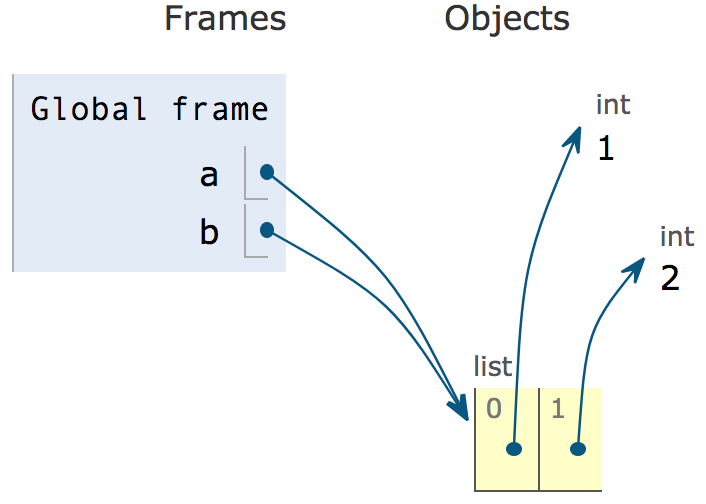
\includegraphics[width=2.25in]{data/a_b_list.png}
  \end{minipage}
  \pause
  \begin{itemize}
  \item \typ{a} is a name for the object \typ{[1, 2]}
  \item \typ{b} is also a name for the \alert{same object}
  \item Changing the contents of \typ{a} reflect in \typ{b}
  \end{itemize}
\end{frame}


\begin{frame}[fragile]
  \frametitle{Names and objects ...}
  \begin{minipage}{0.4\textwidth}
  \begin{lstlisting}
In []: a.append(3)

In []: b
Out[]: [1, 2, 3]
  \end{lstlisting}
\end{minipage}
  \begin{minipage}{0.4\textwidth}
    \hspace*{0.4in}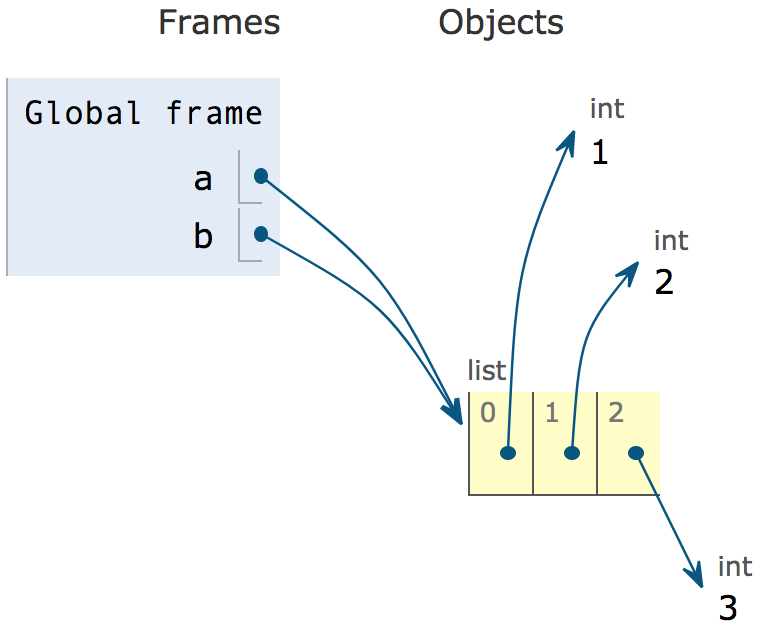
\includegraphics[width=2.25in]{data/a_b_list1.png}
  \end{minipage}

\end{frame}

\begin{frame}[fragile]
  \frametitle{Names and objects ...}
  \begin{minipage}{0.4\textwidth}
  \begin{itemize}
  \item Re-assign \typ{a}
  \end{itemize}
  \begin{lstlisting}
In []: a = 'hello'
\end{lstlisting}
\pause
\end{minipage}
  \begin{minipage}{0.4\textwidth}
    \hspace*{0.4in}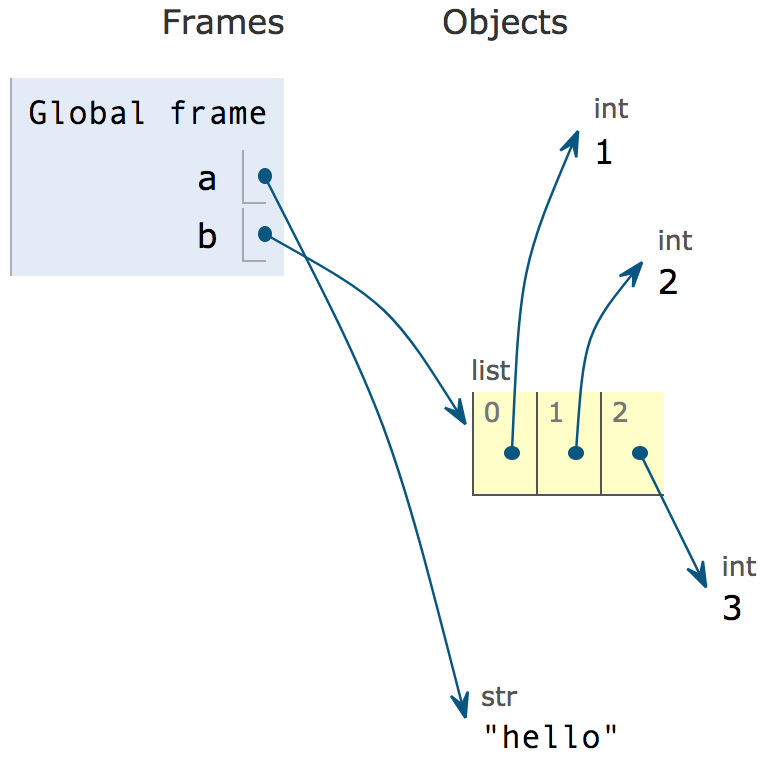
\includegraphics[width=2.25in]{data/a_str_b_list.png}
  \end{minipage}
\end{frame}

\begin{frame}[fragile]
  \frametitle{Names and objects ...}
  Rendered more compactly:
  \vspace*{0.25in}
  \begin{center}
    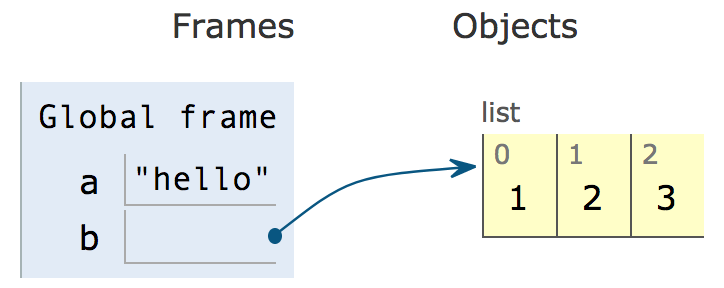
\includegraphics[width=3in]{data/a_str_b_list_compact.png}
  \end{center}
  \vspace*{0.5in}
  {\small Made with: \url{pythontutor.com}}
\end{frame}

\begin{frame}
  \frametitle{Summary}
  \begin{itemize}
  \item Expressions: evaluate to something
  \item Statements: instruct Python to do something
  \item Objects: identity, type, value
  \item Assignments bind names to objects
  \item Frame: an environment for bindings
  \item Explore \url{pythontutor.com}
  \end{itemize}
\end{frame}

\begin{frame}[fragile]
  \frametitle{Exercise 1}
\begin{lstlisting}
a = [1, 2]
b = a
c = [10, 20]
a.append(c)
del b
c.append(30)
del c
a[-1].append(40)
a = 1
\end{lstlisting}
\vspace*{0.1in}
  \begin{itemize}
  \item Run step-by-step on \url{pythontutor.com}
  \item Predict the output before you see the answer
  \end{itemize}
\end{frame}

\begin{frame}[fragile]
  \frametitle{Exercise 2}
\begin{lstlisting}
a = [1, 2]
c = [10, 20]
a.append(c)

c.append(a)
a.append(a)
\end{lstlisting}
\vspace*{0.1in}

  \begin{itemize}
  \item Run step-by-step on \url{pythontutor.com}
  \item Predict the output before you see the answer
  \end{itemize}
\end{frame}

\begin{frame}[fragile]
  \frametitle{Exercise 3}
\begin{lstlisting}
x = [1, 2]
y = 'hello'

def f(x):
   y = x + 1
   return x*y

f(2)
\end{lstlisting}
\vspace*{0.1in}
  \begin{itemize}
  \item Run step-by-step on \url{pythontutor.com}
  \item Predict the output before you see the answer
  \end{itemize}

\end{frame}

\begin{frame}[fragile]
  \frametitle{Exercise 4}
\begin{lstlisting}
def f(x):
    def g(x):
        return x + 1
    return g(x)

f(1)
f(2)
\end{lstlisting}
\vspace*{0.1in}
  \begin{itemize}
  \item Run step-by-step on \url{pythontutor.com}
  \item Predict the output before you see the answer
  \end{itemize}

\end{frame}

\begin{frame}[fragile]
  \frametitle{Exercise 5}
\begin{lstlisting}
def mul(x):
    def g(y):
        return y*x
    return g

twice = mul(2.0)
twice(20)
\end{lstlisting}
\vspace*{0.1in}
  \begin{itemize}
  \item Run step-by-step on \url{pythontutor.com}
  \item Predict the output before you see the answer
  \end{itemize}

\end{frame}


\end{document}
